\documentclass[avery5371, grid,frame]{flashcards}

\usepackage{graphicx}
\usepackage{geometry}

\geometry{a4paper, landscape}
\cardfrontstyle[\large\slshape]{headings}
\cardbackstyle{empty}

\begin{document}

\renewcommand{\cardpaper}{a4paper}
\renewcommand{\cardpapermode}{landscape}
\renewcommand{\cardrows}{2}
\renewcommand{\cardcolumns}{2}
\setlength{\cardheight}{3.5in}
\setlength{\cardwidth}{5.0in}
\setlength{\topoffset}{0.65in}
\setlength{\oddoffset}{0.65in}
\setlength{\evenoffset}{0.65in}

\begin{flashcard}{hard}
    \vspace*{\fill}
    \begin{center}
        \begin{minipage}[c]{.45\textwidth}
            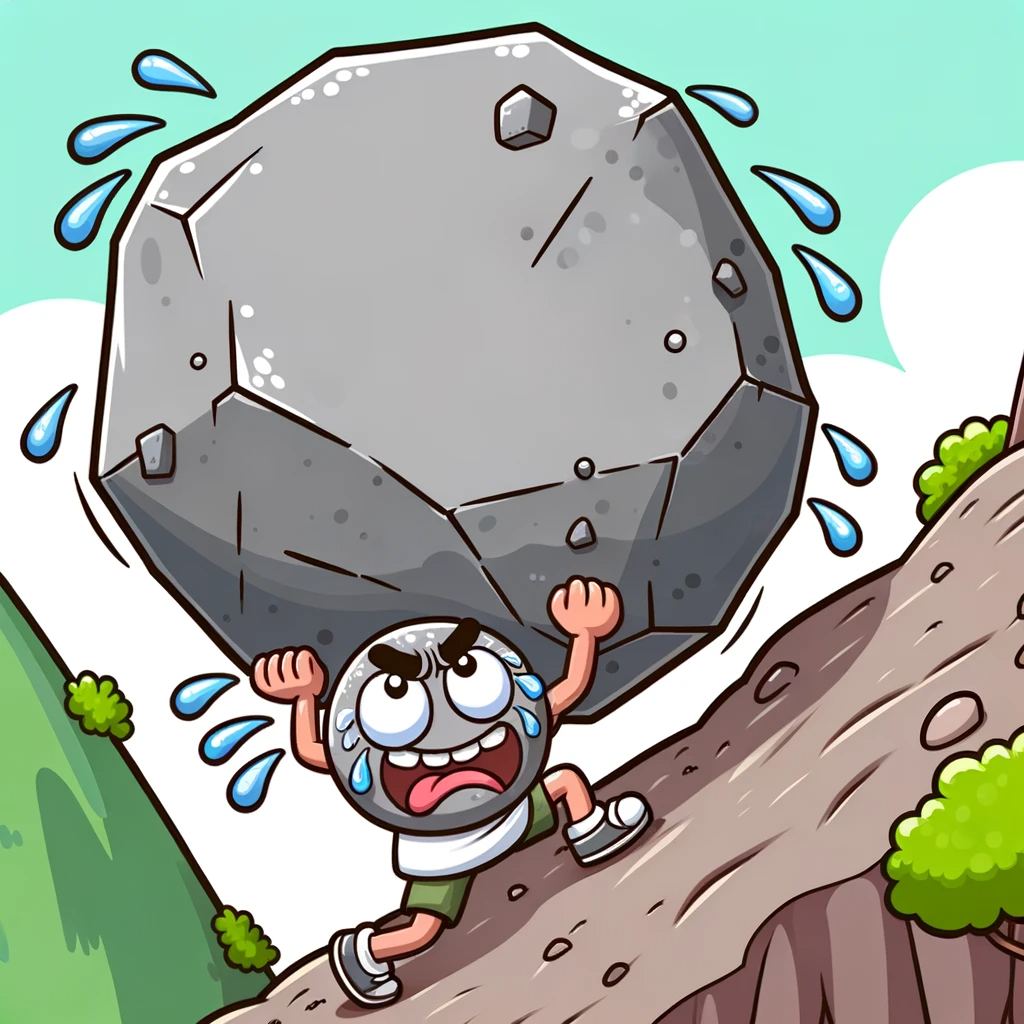
\includegraphics[width=\textwidth]{cards/h/hard/hard - a character struggling to push a massive boulder up a steep hill, beads of sweat on their forehead.png}
        \end{minipage}
        \begin{minipage}[c]{.45\textwidth}
            \begin{itemize}\setlength\itemsep{12pt}
            \item Explanation: \ Difficult to do or understanding

            \item Example: \ a character struggling to push a massive boulder up a steep hill, beads of sweat on their forehead
            \end{itemize}
        \end{minipage}
    \end{center}
    \vspace*{\fill}
\end{flashcard}\begin{flashcard}{hard}
    \vspace*{\fill}
    \begin{center}
        \begin{minipage}[c]{.45\textwidth}
            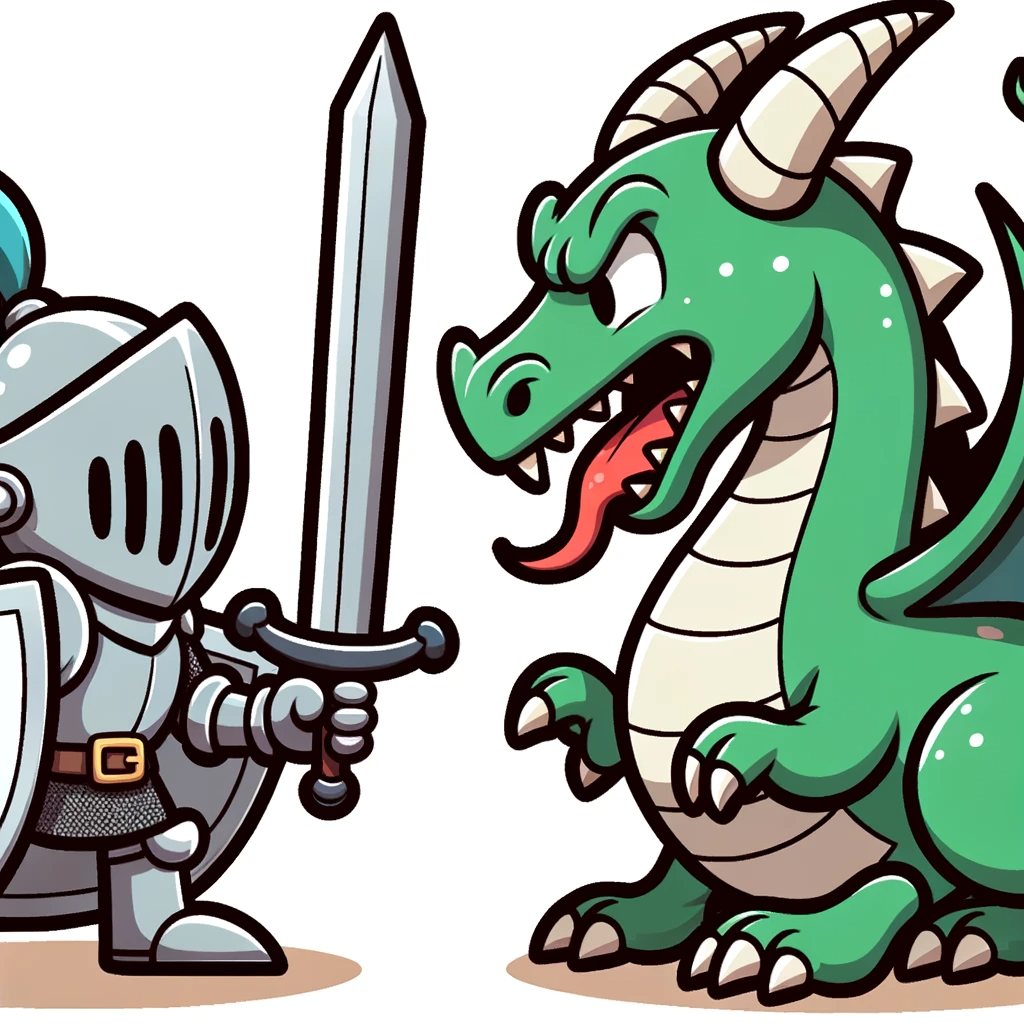
\includegraphics[width=\textwidth]{cards/h/hard/hard - a knight facing a fierce dragon, holding a shield and sword, ready for a challenging battle.png}
        \end{minipage}
        \begin{minipage}[c]{.45\textwidth}
            \begin{itemize}\setlength\itemsep{12pt}
            \item Explanation: \ Difficult to do or understanding

            \item Example: \ a knight facing a fierce dragon, holding a shield and sword, ready for a challenging battle
            \end{itemize}
        \end{minipage}
    \end{center}
    \vspace*{\fill}
\end{flashcard}\begin{flashcard}{hard}
    \vspace*{\fill}
    \begin{center}
        \begin{minipage}[c]{.45\textwidth}
            
\includegraphics[width=\textwidth]{cards/h/hard/hard - a student scratching their head, surrounded by piles of books, trying to solve a complex math problem on a chalkboard.png}
        \end{minipage}
        \begin{minipage}[c]{.45\textwidth}
            \begin{itemize}\setlength\itemsep{12pt}
            \item Explanation: \ Difficult to do or understanding

            \item Example: \ a student scratching their head, surrounded by piles of books, trying to solve a complex math problem on a chalkboard
            \end{itemize}
        \end{minipage}
    \end{center}
    \vspace*{\fill}
\end{flashcard}\begin{flashcard}{hard}
    \vspace*{\fill}
    \begin{center}
        \begin{minipage}[c]{.45\textwidth}
            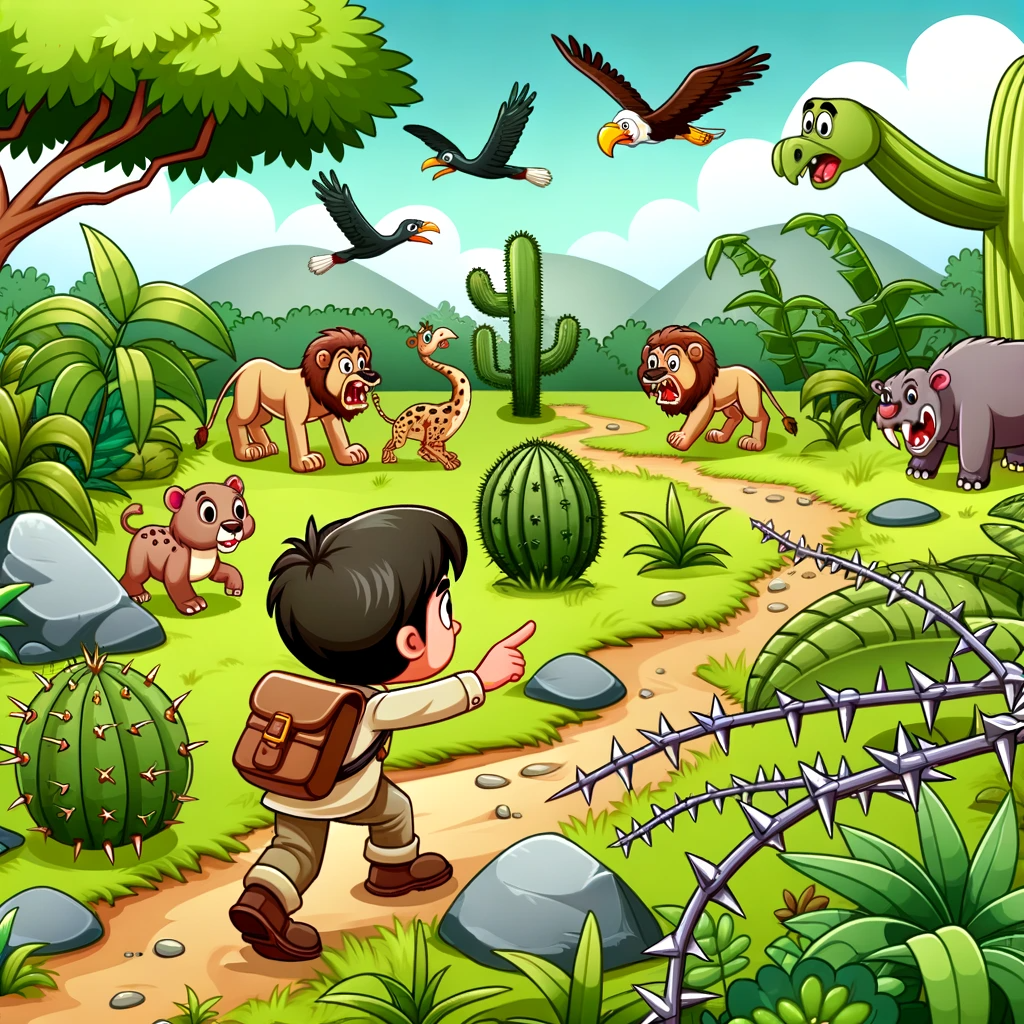
\includegraphics[width=\textwidth]{cards/h/hard/hard - an explorer in a dense jungle, facing various obstacles like wild animals and thorny plants, determined to find their way.png}
        \end{minipage}
        \begin{minipage}[c]{.45\textwidth}
            \begin{itemize}\setlength\itemsep{12pt}
            \item Explanation: \ Difficult to do or understanding

            \item Example: \ an explorer in a dense jungle, facing various obstacles like wild animals and thorny plants, determined to find their way
            \end{itemize}
        \end{minipage}
    \end{center}
    \vspace*{\fill}
\end{flashcard}

\end{document}